\begin{figure}[!ht]
	\centering
	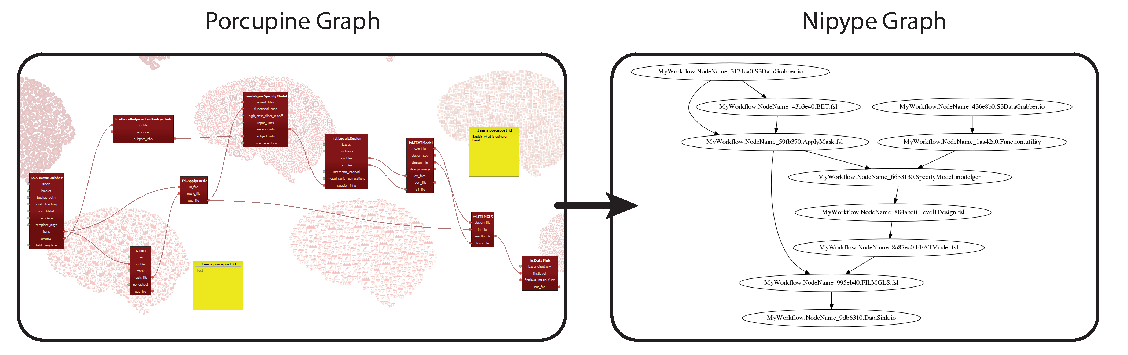
\includegraphics[width=0.9\textwidth, clip=true]{./Chapters/05_Porcupine/./Images/pork_graph.pdf}
	\caption{An example of a more complicated and realistic fMRI preprocessing pipeline. Once the code is generated, this can in turn be transformed into a Nipype graph visualisation. Whereas this is usually the end point for a pipeline in Nipype, we here propose to use a visualisation as a starting point of one's analysis.}
	\label{fig:porcupine-advanced}
\end{figure}